\subsection{Development View}

\subsubsection{Package Diagram}

The following package diagram presents the modular decomposition of the F-LOW system. It illustrates how the system is organized into high-level packages, each encapsulating a major responsibility within the architecture.

\begin{figure}[H]
    \centering
    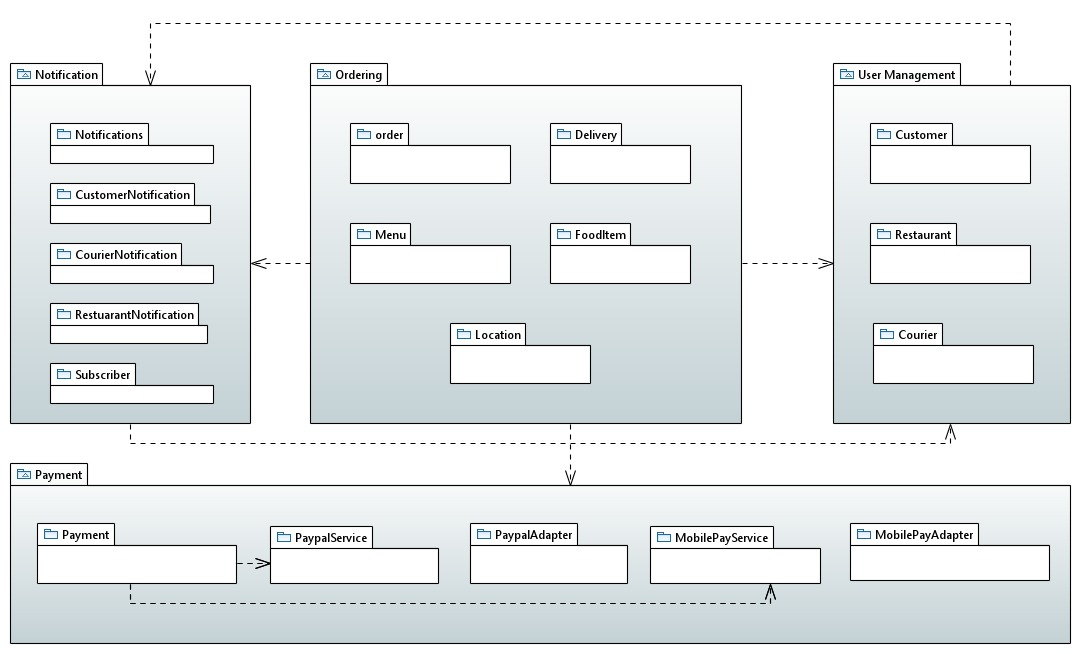
\includegraphics[width=0.9\textwidth]{FIGS/PackageDiagram.jpg}
    \caption{Package Diagram of the F-LOW System}
\end{figure}

Each package encapsulates a specific aspect of the system:

\begin{enumerate}
    \item \textbf{User Management}: Manages user entities such as \texttt{Customer}, \texttt{Courier}, and \texttt{Restaurant}. These entities serve as primary actors throughout the system.
    \item \textbf{Ordering}: Handles business logic for placing, updating, and tracking orders. It integrates food items, menus, delivery logistics, and location services.
    \item \textbf{Payment}: Defines the abstract interface for handling transactions. It supports adapters for multiple services (e.g., PayPal, MobilePay) via the Adapter pattern.
    \item \textbf{Notification}: Implements an event-based architecture using the Observer pattern. It sends updates to users based on state changes in ordering or delivery.
\end{enumerate}

\paragraph{\textbf{\texttt{<<import>>}} Dependencies:}The following relationships are modeled using the \texttt{<<import>>} stereotype to indicate a strong dependency at the interface level:\\
\textbf{Ordering $\rightarrow$ User Management}: Order components directly reference entities such as \texttt{Customer}, \texttt{Courier}, and \texttt{Restaurant} to bind orders to users.\\
\textbf{Ordering $\rightarrow$ Payment}: The \texttt{Order} logic calls the \texttt{pay(info, provider)} method provided by the \texttt{Payment} interface.\\
\textbf{User Management $\rightarrow$ Notification}: Actors like \texttt{Customer}, \texttt{Restaurant}, and \texttt{Courier} subscribe to notification events for receiving system updates.\\
\textbf{Ordering $\rightarrow$ Notification}: Classes such as \texttt{Order} and \texttt{Delivery} generate notifications, relying on \texttt{Notification} and \texttt{Subscriber} components.

\paragraph{Plain Dependencies:}Dashed arrows without stereotypes indicate looser coupling where only selected types are referenced without full namespace import:\\
\textbf{Payment $\dashrightarrow$ PaypalService / MobilePayService}: These services are specific implementations used internally by their respective adapters; they are not exposed system-wide.\\
\textbf{Notification $\dashrightarrow$ User Management}: Notification components may reference actor instances to deliver updates, but do not rely on their full interfaces or APIs.

This separation of concerns through modular packaging ensures extensibility, minimizes coupling, and enables cohesive subsystem development aligned with sound architectural principles.
